\documentclass[12pt,a4paper,oneside]{report}
\usepackage[utf8]{inputenc}

\usepackage{enumerate}
\usepackage{amsmath}
\usepackage{amssymb}
\usepackage{graphicx}
\usepackage{subfigure}
\usepackage[left=3cm,right=3cm,top=3cm,bottom=4cm]{geometry}
\usepackage{caption}
\usepackage{indentfirst}
\usepackage{multirow}
\usepackage{titlesec}
\usepackage{indentfirst}
\usepackage{cite}
\usepackage{algorithm}  
\usepackage{algorithmicx}  
\usepackage{algpseudocode}
\usepackage{tikz}
\usetikzlibrary{arrows}
\usetikzlibrary{snakes}
\usepackage{setspace}
\usepackage{booktabs}
\usepackage{CJK}

\usepackage{minted}
\newcommand{\inputmintedindent}[2]{
    \begin{minipage}{0.1\linewidth}\end{minipage}
    \begin{minipage}{0.85\linewidth}
        \inputminted[linenos,breaklines,fontsize=\footnotesize]{#1}{#2}
    \end{minipage}\\[0.5em]
}


\renewcommand{\algorithmicrequire}{\textbf{Input:}}  
\renewcommand{\algorithmicensure}{\textbf{Output:}}  

\renewcommand{\thechapter}{\Roman{chapter}}
\titleformat{\chapter}{\Huge\bfseries}{\thechapter}{0.5em}{}
\renewcommand{\thesection}{  \arabic{section}}


\author{
    \textbf{Joint Authors:}\\
    Gu Yichen 5143709162\\
    Liu Yihao 515370910207\\
    Peng Junda 5133\\
    Wang Dayi 5133\\
    \normalsize{(In Alphabetic Order)}\\
    \\
    \textbf{Instructor:}\\
    Prof. Charlemagne Manuel\\ \\ \textbf{Course:}\\VE475\\ Introduction to Cryptography\\ \\ \textbf{Institute:}\\University of Michigan - Shanghai Jiao Tong University\\Joint Institute}
\title{\textbf{Project:\\Hash Functions}}

\date{2017-August-8th}

\begin{document}
\maketitle

\begin{abstract}

The goal of this project is to perform some personal study in order to acquire the extra knowledge in cryptography while also improving major skills such as writing, collaboration and public presentation. In this project, we intend to have a preliminary understanding of a method of cryptography: Hash Functions.\\

In this project, we first . Then in the second chapter. The third chapter is mainly about. In the fourth chapter.\\

Cryptography is quite a complex and esoteric subject and there are so many mysteries in the world. We just do a simple and shallow survey on the aspect of Hash Functions. There still remains a large number of interesting and profound problems to be solved. The study of cryptography is still pending.\\

\end{abstract}


\tableofcontents
\chapter{  Introduction}

\chapter{KECCAK-$p$ Permutations}
The KECCAK-$p$ permutations are specified with two parameters:
\begin{itemize}
    \item One is the fixed length of the strings that are permuted, called the $width$ of the permutation, denoted by $b$.
    \item The other is the number of iterations of an internal transformation, called a $round$, denoted by $n_r$.
\end{itemize}

The KECCAK-$p$ permutation with $n_r$ rounds and width $b$ is denoted by KECCAK-$p[b, n_r]$ and the permutation is defined for any $b$ in $\{25,50,100,200,400,800,1600\}$ and any positive integer $n_r$.\\

A round of a KECCAK-$p$ permutation, denoted by Rnd, consists of a sequence of five transformations, which are called the $step\ mappings$. The permutation is specified in terms of an array of values for $b$ bits that is repeatedly updated, called the $state$. The state is initially set to the input values of the permutation.

\section{State}
The state for the KECCAK-$p[b, n_r]$ permutation is comprised of $b$ bits. There are two other quantities: $w=b/25$ and $l=\log_2 (b/25)$. The seven possible values for these variables that are defined for the KECCAK-$p$ permutations are given in the following table.

\begin{table}[H]
  \centering
  \caption{KECCAK-$p$ permutation widths and related quantities}
    \begin{tabular}{cccccccc}
    \toprule
    b & 25 & 50 & 100 & 200 & 400 & 800 & 1600 \\
    \midrule
    w & 1 & 2 & 4 & 8 & 16 & 32 & 64 \\
    \midrule
    l & 0 & 1 & 2 & 3 & 4 & 5 & 6 \\
    \bottomrule
    \end{tabular}
\end{table}%

It is convenient to represent the input and output states of the permutation as $b$-bit strings, and to represent the input and output states of the step mappings as 5-by-5-by-$w$ arrays of bits. If $S$ denotes a string that represents the state, then its bits are indexed from 0 to $b–1$, so that
$$S=S[0] \mid\mid S[1] \mid\mid \cdots \mid\mid S[b-2] \mid\mid S[b-1]$$

If $A$ denotes a 5-by-5-by-$w$ array of bits that represents the state, then its indices are the integer triples $(x,y,z)$ for which $0 \leq x < 5$, $0 \leq y < 5$ and $0 \leq z < w$. The bit corresponding to $(x,y,z)$ is denoted by $A[x,y,z]$. A $state\ array$ is a representation of the state by a three-dimensional array that is indexed in this manner.

\subsection{State Array}
\begin{figure}[H]
\centering
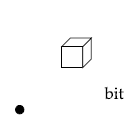
\includegraphics[width=1.5in]{imgs/origin.png}
\caption{Original Part of State Array} 
\end{figure}

\begin{figure}[H]
\begin{minipage}[t]{0.3\linewidth} 
\centering 
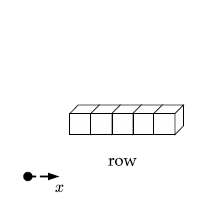
\includegraphics[width=2in]{imgs/1D1.png} 
\end{minipage}
\begin{minipage}[t]{0.3\linewidth} 
\centering 
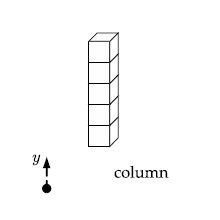
\includegraphics[width=2in]{imgs/1D2.png} 
\end{minipage}
\begin{minipage}[t]{0.3\linewidth} 
\centering 
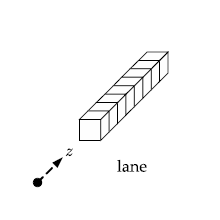
\includegraphics[width=2in]{imgs/1D3.png} 
\end{minipage}
\caption{1-D Parts of State Array} 
\end{figure}

\begin{figure}[H]
\begin{minipage}[t]{0.3\linewidth} 
\centering 
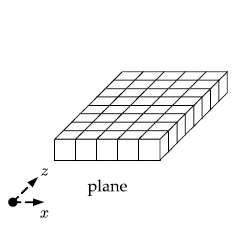
\includegraphics[width=1.8in]{imgs/2D1.png} 
\end{minipage}
\begin{minipage}[t]{0.3\linewidth} 
\centering 
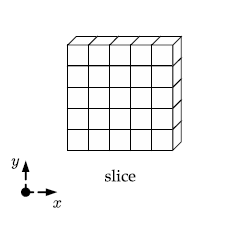
\includegraphics[width=1.8in]{imgs/2D2.png} 
\end{minipage}
\begin{minipage}[t]{0.3\linewidth} 
\centering 
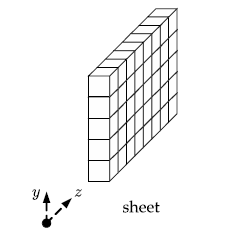
\includegraphics[width=1.8in]{imgs/2D3.png} 
\end{minipage}
\caption{2-D Parts of State Array} 
\end{figure}

\begin{figure}[H]
\centering
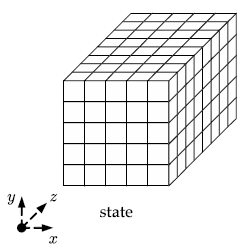
\includegraphics[width=1.5in]{imgs/3D.png}
\caption{3-D Part of State Array} 
\end{figure}

For $b=200 (w=b/25=8)$, the state array for a KECCAK-$p$ permutation and its lower-dimensional sub-arrays are illustrated in figures above. For a state, the single-dimensional sub-arrays are called $rows$, $columns$ and $lanes$. The two-dimensional sub-arrays are called $sheets$, $planes$ and $slices$. The original sub-array is called $bit$.

\subsection{Converting Strings to State Arrays}
$S$ is a string of $b$ bits that represents the state for the KECCAK-$p[b, n_r]$ permutation. The corresponding state array $A$ is defined as follows:\\
$$\rm{For\ all\ triples\ (x,y,z)\ such\ that\ 0 \leq x < 5,\ 0 \leq y < 5\ and\ 0 \leq z < w}$$
$$A[x,y,z]=S[w(5y+x)+z]$$

\inputmintedindent{C}{code_split/sha3_convert_string_to_state_array.c}

\subsection{Converting State Arrays to Strings}
$A$ is a state array and the corresponding string representation $S$ can be constructed from the lanes and planes of $A$, as follows:\\

For each pair of integers $(i,j)$ such that $0 \leq i < 5$ and $0 \leq j < 5$:
$$Lane(i,j)=A[i,j,0] \mid\mid A[i,j,1] \mid\mid \cdots \mid\mid A[i,j,w-2] \mid\mid A[i,j,w-1]$$

For each integer $j$ such that $0 \leq j < 5$:
$$Plane(j)=Lane(0,j) \mid\mid Lane(1,j) \mid\mid Lane(2,j) \mid\mid Lane(3,j) \mid\mid Lane(4,j)$$

Then we can have the corresponding string representation $S$: 
$$S=Plane(0) \mid\mid Plane(1) \mid\mid Plane(2) \mid\mid Plane(3) \mid\mid Plane(4)$$

\inputmintedindent{C}{code_split/sha3_convert_state_array_to_string.c}


\newpage
\subsection{Labeling Convention for the State Array}
In the diagrams of the state that accompany the specifications of the step mappings, the lane that corresponds to the coordinates $(x,y)=(0,0)$ is depicted at the center of the slices. The complete labeling of the $(x,y,z)$ coordinates for those diagrams is shown in the following figure.

\begin{figure}[H]
\centering
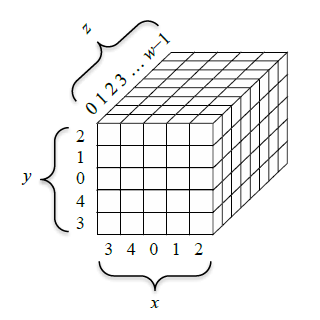
\includegraphics[width=2in]{imgs/xyz.png}
\caption{The $(x,y,z)$ coordinates for the diagrams of the step mappings} 
\end{figure}

\section{Step Mappings}
The five step mappings that comprise a round of KECCAK-$p[b, n_r]$ are denoted by $\theta$, $\rho$, $\pi$, $\chi$ and $\imath$. The algorithm for each step mapping takes a state array $A$ as the input and returns an updated state array $A^{'}$ as the output. The size of the state is a parameter that is omitted from the notation, because $b$ is always specified when the step mappings are invoked.

\subsection{Specification of $\theta$}
\begin{algorithm}[H]
    \begin{algorithmic}
        \Require \\
        state array $A$
        \Ensure \\
        state array $A^{'}$
        \Function {$\theta$}{$A$}
            \For {all pairs $(x,z)$ such that $0 \leq x < 5$ and $0 \leq z < w$}  
                \State $C[x,z]=A[x,0,z] \oplus A[x,1,z] \oplus A[x,2,z] \oplus A[x,3,z] \oplus A[x,4,z]$
                \State $D[x,z]=C[(x-1)$ mod $5,z] \oplus C[(x+1)$ mod $5, (z-1)$ mod $w]$
            \EndFor
            \For {all triples $(x,y,z)$ such that $0 \leq x < 5$, $0 \leq y < 5$ and $0 \leq z < w$}  
                \State $A^{'}[x,y,z]=A[x,y,z] \oplus D[x,z]$
            \EndFor
            \State \Return{state array $A^{'}$}  
        \EndFunction  
    \end{algorithmic}  
\end{algorithm}


\inputmintedindent{C}{code_split/sha3_step_theta.c}


\subsection{Specification of $\rho$}
\begin{algorithm}[H]
    \begin{algorithmic}
        \Require \\
        state array $A$
        \Ensure \\
        state array $A^{'}$
        \Function {$\rho$}{$A$}
            \For {all $z$ such that $0 \leq z < w$}  
                \State $A^{'}[0,0,z]=A[0,0,z]$
            \EndFor
            \State $(x,y)=(1,0)$
            \For {$t=0$ to $23$}  
                \For {all $z$ such that $0 \leq z < w$} 
                    \State $A^{'}[x,y,z]=A[x,y,(z-\dfrac{(t+1)(t+2)}{2})$ mod $w]$
                \EndFor
                \State $(x,y)=(y,(2x+3y)$ mod $5)$
            \EndFor
            \State \Return{state array $A^{'}$}  
        \EndFunction  
    \end{algorithmic}  
\end{algorithm}

\inputmintedindent{C}{code_split/sha3_step_rho.c}


\subsection{Specification of $\pi$}
\begin{algorithm}[H]
    \begin{algorithmic}
        \Require \\
        state array $A$
        \Ensure \\
        state array $A^{'}$
        \Function {$\pi$}{$A$}
            \For {all triples $(x,y,z)$ such that $0 \leq x < 5$, $0 \leq y < 5$ and $0 \leq z < w$}
               \State $A^{'}[x,y,z]=A[(x+3y)$ mod $5,x,z]$
            \EndFor
            \State \Return{state array $A^{'}$}  
        \EndFunction  
    \end{algorithmic}  
\end{algorithm}

\inputmintedindent{C}{code_split/sha3_step_pi.c}


\subsection{Specification of $\chi$}
\begin{algorithm}[H]
    \begin{algorithmic}
        \Require \\
        state array $A$
        \Ensure \\
        state array $A^{'}$
        \Function {$\chi$}{$A$}
            \For {all triples $(x,y,z)$ such that $0 \leq x < 5$, $0 \leq y < 5$ and $0 \leq z < w$}
                \State $A^{'}[x,y,z]=A[x,y,z] \oplus ((A[(x+1)$ mod $5,x,z] \oplus 1) \cdot A[(x+2)$ mod $5,y,z])$
            \EndFor
            \State \Return{state array $A^{'}$}  
        \EndFunction  
    \end{algorithmic}  
\end{algorithm}

\inputmintedindent{C}{code_split/sha3_step_chi.c}

\subsection{Specification of $\iota$}
\begin{algorithm}[H]
    \begin{algorithmic}
        \Require \\
        integer $t$
        \Ensure \\
        bit $rc(t)$
        \Function {$rc$}{$t$}
            \If {$t$ mod $255=0$}
                \State \Return{$1$}
            \EndIf
            \State $R=10000000$
                \For {$i=1$ to $t$ mod $255$}
                    \State $R=0 \mid\mid R$
                    \State $R[0]=R[0] \oplus R[8]$
                    \State $R[4]=R[4] \oplus R[8]$
                    \State $R[5]=R[5] \oplus R[8]$
                    \State $R[6]=R[6] \oplus R[8]$
                    \State $R=$Trunc$_8 [R]$
                \EndFor
                \State \Return{$R[0]$}  
        \EndFunction  
    \end{algorithmic}  
\end{algorithm}

\inputmintedindent{C}{code_split/sha3_generate_rc.c}


\begin{algorithm}[H]
    \begin{algorithmic}
        \Require \\
        state array $A$
        round index $i_r$
        \Ensure \\
        state array $A^{'}$
        \Function {$\chi$}{$A$}
            \For {all triples $(x,y,z)$ such that $0 \leq x < 5$, $0 \leq y < 5$ and $0 \leq z < w$}
                \State $A^{'}[x,y,z]=A[x,y,z]$
            \EndFor
            \State $RC=0^w$
            \For {$j=0$ to $l$}
                \State $RC[2^j-1]=rc(j+7i_r)$
            \EndFor
            \For {all $z$ such that $0 \leq z < w$}
                \State $A^{'}[0,0,z]=A^{'}[0,0,z] \oplus RC[z]$
            \EndFor
            \State \Return{state array $A^{'}$}  
        \EndFunction  
    \end{algorithmic}  
\end{algorithm}

\inputmintedindent{C}{code_split/sha3_step_iota.c}


\section{KECCAK-$p[b, n_r]$}



\chapter{KECCAK}
\section{Specification of pad10*1}
\section{Specification of KECCAK$[c]$}

\chapter{  Conclusion and Discussion}
\section{Discussion}
In this project, we have searched a lot about the Hash Functions. In brief, our team learned a lot according to this project, and expand one's horizon on the vast field of cryptography.\\

\section{Conclusion}
In this project, we have made the study of Hash Functions in order to acquire the extra knowledge in cryptography. What's more, our major skills such as writing and collaboration haven been improved as well. We have had a preliminary understanding of xxx thanks for this subject. We have understood xxx. The superiority of xxx is represented throughout whole the project. Cryptography is quite a complex and esoteric subject and there are so many mysteries in the world. But we still have enough enthusiasm to explore the secrets in the world of cryptography. The study of cryptography is still pending.\\


\chapter{  Bibliography}
\noindent [1] \\

\end{document}
 
